%% beamer-lake-fig.tex
%%
%% Copyright (C) 2016 - 2017  Joseph Stachelek
%%
%% This file is part of beamer-lake-fig repository.
%%
%% beamer-lake-fig is free software: you can redistribute it
%% and/or modify it under the terms of the GNU General Public License as
%% published by the Free Software Foundation, either version 2 of the
%% License, or (at your option) any later version.
%%
%% beamer-lake-fig is distributed in the hope that it will be
%% useful, but WITHOUT ANY WARRANTY; without even the implied warranty of
%% MERCHANTABILITY or FITNESS FOR A PARTICULAR PURPOSE.  See the GNU General
%% Public License for more details.
%%
%% You should have received a copy of the GNU General Public License along with
%% beamer-lake-fig.  If not, see <http://www.gnu.org/licenses/>.

\PassOptionsToPackage{x11names}{xcolor}
\usetikzlibrary{decorations.pathmorphing,calc}

\usepackage{subfiles}
\usepackage{pbox}
\usepackage{multirow}
\usepackage{tabularx}
\usepackage{colortbl}

\usepackage{array}
\newcolumntype{L}[1]{>{\raggedright\let\newline\\\arraybackslash\hspace{0pt}}m{#1}}
\newcolumntype{R}[1]{>{\raggedleft\let\newline\\\arraybackslash\hspace{0pt}}m{#1}}

\def\mystrut(#1,#2){\vrule height #1 depth #2 width 0pt}

\newcolumntype{C}[1]{%
   >{\mystrut(3ex,2ex)\centering}%
   p{#1}%
   <{}}

\newcolumntype{K}[1]{%
 >{\vbox to 5ex\bgroup\vfill\centering}%
 p{#1}%
 <{\egroup}}

% \definecolor{darkgreen}{rgb}{0.13,0.62,0.25}
\definecolor{darkgreen}{RGB}{14,90,30}

%%%%%%%%%%%%%%%%%%%%%%%%%%%%%%%%%%%%%%%%%%%%%%%%%%%%%%%%%%%%%%%%%%%%%%%%%%%%%%%
\section{lakediagramgreen}
\def\lakediagramgreen[#1]{
\begin{tikzpicture}[scale = #1]
% https://tex.stackexchange.com/questions/95044/create-diagrams-in-latex-with-tikz

% Define some reference points 
% The figure is drawn a bit bigger, and then clipped to the following dimensions:
\coordinate (clipping area) at (10, 7);
\clip (0,0) rectangle (clipping area);

% Next reference points are relative to the lower left corner of the clipping area
\coordinate (water level) at (0, 6);
\coordinate (bottom)      at (5, 1.3);     % (bottom of the pit)
\coordinate (ground1)     at (0, 5);       % (left shore)
\coordinate (ground2)     at (10, 5);      % (right shore)

% Coordinates of the bigger area really drawn
\coordinate (lower left)  at ([xshift=-5mm, yshift=-5mm] 0,0);
\coordinate (upper right) at ([xshift=5mm,  yshift=5mm] clipping area);

% Draw the water and ripples
\draw [draw=blue!80!black, decoration={bumps, mirror, segment length=6mm}, decorate,
     bottom color=cyan!60!black, top color=darkgreen!20!white] 
  (lower left) rectangle (water level-|upper right);

% Draw the ground
\draw [draw=brown!30!black, fill=brown] 
  (lower left) -- (lower left|-ground1)  --
  (ground1) .. controls ($(ground1)!.3!(bottom)$) and (bottom-|ground1) ..
  (bottom) .. controls (bottom-|ground2) and ($(ground2)!.3!(bottom)$) .. 
  (ground2) -- (ground2-|upper right) -- (lower left-|upper right) -- cycle;

% \draw[dotted](0,0) rectangle (clipping area);

% labels
\draw[>=stealth, ->, line width = 0.7mm] (0, 5.5) -- (3, 5.5) node at (1.5, 4.8) {Inputs};
\draw[>=stealth, ->, line width = 0.2mm] (8, 5.5) -- (10, 5.5) node at (8.5, 4.8) {Outputs};

\end{tikzpicture}
}

\section{lakediagramblue}
\def\lakediagramblue[#1]{
\begin{tikzpicture}[scale = #1]
% https://tex.stackexchange.com/questions/95044/create-diagrams-in-latex-with-tikz

% Define some reference points 
% The figure is drawn a bit bigger, and then clipped to the following dimensions:
\coordinate (clipping area) at (10, 7);
\clip (0,0) rectangle (clipping area);

% Next reference points are relative to the lower left corner of the clipping area
\coordinate (water level) at (0, 6);
\coordinate (bottom)      at (5, 1.3);     % (bottom of the pit)
\coordinate (ground1)     at (0, 5);       % (left shore)
\coordinate (ground2)     at (10, 5);      % (right shore)

% Coordinates of the bigger area really drawn
\coordinate (lower left)  at ([xshift=-5mm, yshift=-5mm] 0,0);
\coordinate (upper right) at ([xshift=5mm,  yshift=5mm] clipping area);

% Draw the water and ripples
\draw [draw=blue!80!black, decoration={bumps, mirror, segment length=6mm}, decorate,
     bottom color=cyan!60!black, top color=blue!20!white] 
  (lower left) rectangle (water level-|upper right);

% Draw the ground
\draw [draw=brown!30!black, fill=brown] 
  (lower left) -- (lower left|-ground1)  --
  (ground1) .. controls ($(ground1)!.3!(bottom)$) and (bottom-|ground1) ..
  (bottom) .. controls (bottom-|ground2) and ($(ground2)!.3!(bottom)$) .. 
  (ground2) -- (ground2-|upper right) -- (lower left-|upper right) -- cycle;

% \draw[dotted](0,0) rectangle (clipping area);

% labels
\draw[>=stealth, ->, line width = 0.5mm] (0, 5.5) -- (3, 5.5) node at (1.5, 4.8) {Inputs};
\draw[>=stealth, ->, line width = 0.5mm] (8, 5.5) -- (10, 5.5) node at (8.5, 4.8) {Outputs};

\end{tikzpicture}
}

%%%%%%%%%%%%%%%%%%%%%%%%%%%%%%%%%%%%%%%%%%%%%%%%%%%%%%%%%%%%%%%%%%%%%%%%%%%%%%%
\section{connectivitydiagram}
\def\connectivitydiagram[#1]{
\begin{columns}

\begin{column}{0.25\textwidth}
    \begin{tikzpicture}[scale = #1]
      \draw [-,ultra thick, cyan] (-1,3) to [out=270,in=180] (0.2,2) to [out=0,in=90] (0,0.3) to [out=90,in=0] (0,-1) to [out=90,in=0] (0.2,-2) to [out=180,in=90] (-1,-3);
      \draw[cyan, ultra thick, domain=0:350, smooth cycle, fill=cyan,yshift=20] plot (\x:0.5+rnd*0.25);
      \draw[cyan, ultra thick, domain=0:350, smooth cycle, fill=cyan,yshift=-50] plot (\x:0.8+rnd*0.5);
      \node at (0,-1.7) {Secondary};
    \end{tikzpicture}
  \end{column}
  
  \begin{column}{0.25\textwidth}
    \begin{tikzpicture}[scale = #1]
      \draw [-,ultra thick, cyan] (-1,3) to [out=270,in=180] (0.2,2) to [out=0,in=90] (0,0);
      \draw[cyan, ultra thick, domain=0:350, smooth cycle, fill=cyan] (0,-3) plot (\x:1+rnd*0.5);
      \node at (0, 0) {Primary};
    \end{tikzpicture}
  \end{column}
  
  \begin{column}{0.25\textwidth}
  \begin{tikzpicture}[scale = #1]
      \draw [-,ultra thick, cyan] (0,0) to [out=90,in=0] (0.2,-2) to [out=180,in=90] (-1,-3);
      \draw[cyan, ultra thick, domain=0:350, smooth cycle, fill=cyan] (0,3) plot (\x:1+rnd*0.5);
      \node at (0, 0) {Headwater};
    \end{tikzpicture}
  \end{column}
  
  \begin{column}{0.25\textwidth}
    \begin{tikzpicture}[scale = #1]
      \draw[cyan, ultra thick, domain=0:350, smooth cycle, fill=cyan] plot (\x:1+rnd*0.5);
      \node at (0, 0) {Isolated};
    \end{tikzpicture}
  \end{column}
  
\end{columns}

}

%%%%%%%%%%%%%%%%%%%%%%%%%%%%%%%%%%%%%%%%%%%%%%%%%%%%%%%%%%%%%%%%%%%%%%%%%%%%%%%
\section{secondaryprofile}
\def\secondaryprofile[#1]#2{
\begin{tikzpicture}[scale = #1]
  \draw [-,line width = 5, #2!100!black] (0.9,0) to [out=0,in=180] (1.55,0);
  \draw [-,line width = 5, dashed, #2!100!black] (5.5,0) to [out=0,in=180] (6.2,0);
  % \node at (2, 1) {Secondary};
\fill[
  top color=#2!100,
  bottom color=#2!40,
  shading=axis,
  opacity=0.45
  ] 
  (0,0) circle (1cm and 0.25cm);
\fill[
  left color=#2!50!black,
  right color=#2!50!black,
  middle color=#2!100,
  shading=axis,
  opacity=0.25
  ] 
  (1,0) {[rounded corners=45pt] -- (0,-2)} -- (-1,0) arc (180:360:1cm and 0.25cm);
  
\fill[
  top color=#2!100,
  bottom color=#2!40,
  shading=axis,
  opacity=0.45,
  xshift=100
  ] 
  (0,0) circle (2cm and 0.5cm);
\fill[
  left color=#2!50!black,
  right color=#2!50!black,
  middle color=#2!100,
  shading=axis,
  opacity=0.25,
  xshift=100
  ] 
  (2,0) {[rounded corners=45pt] -- (0,-3)} -- (-2,0) arc (180:360:2cm and 0.5cm);
\end{tikzpicture}
}

%%%%%%%%%%%%%%%%%%%%%%%%%%%%%%%%%%%%%%%%%%%%%%%%%%%%%%%%%%%%%%%%%%%%%%%%%%%%%%%
\section{secondaryprofileflatequal}
\def\secondaryprofileflatequal[#1]#2{
\begin{tikzpicture}[scale = #1]
  \draw [fill=#2, ultra thick] (0.1,-.3) rectangle (1.7,0.1);
  \draw [fill=#2, ultra thick] (5.3,0.1) rectangle (6.2,-0.3);
  % \node at (2, 1) {Secondary};
\draw
  [fill=#2,
  ultra thick,
  xshift=-50
  ] 
  (0,0) circle (2cm and 0.5cm);
\draw
  [fill=#2,
  ultra thick,
  xshift=-50
  ] 
  (2,0) {[rounded corners=45pt] -- (0,-3)} -- (-2,0) arc (180:360:2cm and 0.5cm);
  
\draw
  [fill = #2,
  ultra thick,
  xshift=100
  ] 
  (0,0) circle (2cm and 0.5cm);
\draw
  [fill = #2,
  ultra thick,
  xshift=100
  ] 
  (2,0) {[rounded corners=45pt] -- (0,-3)} -- (-2,0) arc (180:360:2cm and 0.5cm);
\end{tikzpicture}
}

%%%%%%%%%%%%%%%%%%%%%%%%%%%%%%%%%%%%%%%%%%%%%%%%%%%%%%%%%%%%%%%%%%%%%%%%%%%%%%%
\section{primaryprofileflatequal}
\def\primaryprofileflatequal[#1]#2{
\begin{tikzpicture}[scale = #1]
  \draw [fill=#2, ultra thick] (1.8,-.3) rectangle (3.2,0.1);
  \draw [fill=#2, ultra thick] (-1.8,0.1) rectangle (-3.2,-0.3);
  % \node at (2, 1) {Secondary};
\draw
  [fill=#2,
  ultra thick
  ] 
  (0,0) circle (2cm and 0.5cm);
\clip (-2,-3) rectangle (2,0);
\draw
  [fill=#2,
  ultra thick
  ] 
  (2,0) {[rounded corners=45pt] -- (0,-3)} -- (-2,0) arc (180:360:2cm and 0.5cm);

\end{tikzpicture}
}

%%%%%%%%%%%%%%%%%%%%%%%%%%%%%%%%%%%%%%%%%%%%%%%%%%%%%%%%%%%%%%%%%%%%%%%%%%%%%%%
\section{headwaterprofileflatequal}
\def\headwaterprofileflatequal[#1]#2{
\begin{tikzpicture}[scale = #1]
  \draw [fill=#2, ultra thick] (1.8,-.3) rectangle (3.2,0.1);
  % \node at (2, 1) {Secondary};
\draw
  [fill=#2,
  ultra thick
  ] 
  (0,0) circle (2cm and 0.5cm);
\clip (-2,-3) rectangle (2,0);
\draw
  [fill=#2,
  ultra thick
  ] 
  (2,0) {[rounded corners=45pt] -- (0,-3)} -- (-2,0) arc (180:360:2cm and 0.5cm);

\end{tikzpicture}
}

%%%%%%%%%%%%%%%%%%%%%%%%%%%%%%%%%%%%%%%%%%%%%%%%%%%%%%%%%%%%%%%%%%%%%%%%%%%%%%%
\section{isolatedprofileflatequal}
\def\isolatedprofileflatequal[#1]#2{
\begin{tikzpicture}[scale = #1]
\draw
  [fill=#2,
  ultra thick
  ] 
  (0,0) circle (2cm and 0.5cm);
\clip (-2,-3) rectangle (2,0);
\draw
  [fill=#2,
  ultra thick
  ] 
  (2,0) {[rounded corners=45pt] -- (0,-3)} -- (-2,0) arc (180:360:2cm and 0.5cm);

\end{tikzpicture}
}

%%%%%%%%%%%%%%%%%%%%%%%%%%%%%%%%%%%%%%%%%%%%%%%%%%%%%%%%%%%%%%%%%%%%%%%%%%%%%%%
\section{headwaterprofile}
\def\headwaterprofile[#1]#2{
\begin{tikzpicture}[scale = #1]
  \draw [-,line width = 5, #2!100!black] (1.95,0) to [out=0,in=180] (2.7,0);
  % \node at (0.4, 1) {Headwater};
\fill[
  top color=#2!100,
  bottom color=#2!40,
  shading=axis,
  opacity=0.45
  ] 
  (0,0) circle (2cm and 0.5cm);
\fill[
  left color=#2!50!black,
  right color=#2!50!black,
  middle color=#2!100,
  shading=axis,
  opacity=0.25
  ] 
  (2,0) {[rounded corners=45pt] -- (0,-3)} -- (-2,0) arc (180:360:2cm and 0.5cm);
\end{tikzpicture}
}

%%%%%%%%%%%%%%%%%%%%%%%%%%%%%%%%%%%%%%%%%%%%%%%%%%%%%%%%%%%%%%%%%%%%%%%%%%%%%%%
\section{primaryprofile}
\def\primaryprofile[#1]#2{
\begin{tikzpicture}[scale = #1]
  \draw [-,line width = 5, #2!100!black] (-2,0) to [out=0,in=180] (-2.7,0);
  \draw [-,line width = 5, dashed, #2!100!black] (2,0) to [out=0,in=180] (2.7,0);
  % \node at (0.4, 1) {Primary};
\fill[
  top color=#2!100,
  bottom color=#2!40,
  shading=axis,
  opacity=0.45
  ] 
  (0,0) circle (2cm and 0.5cm);
\fill[
  left color=#2!50!black,
  right color=#2!50!black,
  middle color=#2!100,
  shading=axis,
  opacity=0.25
  ] 
  (2,0) {[rounded corners=45pt] -- (0,-3)} -- (-2,0) arc (180:360:2cm and 0.5cm);
\end{tikzpicture}
}

%%%%%%%%%%%%%%%%%%%%%%%%%%%%%%%%%%%%%%%%%%%%%%%%%%%%%%%%%%%%%%%%%%%%%%%%%%%%%%%
\section{isolatedprofile}
\def\isolatedprofile[#1]#2{
\begin{tikzpicture}[scale = #1]
\fill[
  top color=#2!100,
  bottom color=#2!40,
  shading=axis,
  opacity=0.45
  ] 
  (0,0) circle (2cm and 0.5cm);
\fill[
  left color=#2!50!black,
  right color=#2!50!black,
  middle color=#2!100,
  shading=axis,
  opacity=0.25
  ] 
  (2,0) {[rounded corners=45pt] -- (0,-3)} -- (-2,0) arc (180:360:2cm and 0.5cm);
\end{tikzpicture}
}

%%%%%%%%%%%%%%%%%%%%%%%%%%%%%%%%%%%%%%%%%%%%%%%%%%%%%%%%%%%%%%%%%%%%%%%%%%%%%%%
\section{primaryprofileplus}
\def\primaryprofileplus{
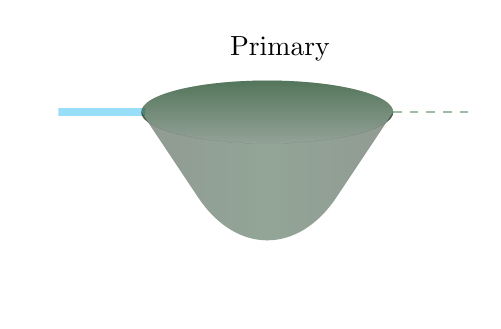
\begin{tikzpicture}[scale = 0.8]
  \draw [-,line width=3pt, cyan!40] (-2,0) to [out=0,in=180] (-3.25,0);
  \draw [-,thick, dashed, darkgreen!40] (2,0) to [out=0,in=180] (3.25,0);
  \node at (0.2, 1) {Primary};
\fill[
  top color=darkgreen!100,
  bottom color=darkgreen!40,
  shading=axis,
  opacity=0.45
  ] 
  (0,0) circle (2cm and 0.5cm);
\fill[
  left color=darkgreen!50!black,
  right color=darkgreen!50!black,
  middle color=darkgreen!100,
  shading=axis,
  opacity=0.25
  ] 
  (2,0) {[rounded corners=45pt] -- (0,-3)} -- (-2,0) arc (180:360:2cm and 0.5cm);
\end{tikzpicture}
}

%%%%%%%%%%%%%%%%%%%%%%%%%%%%%%%%%%%%%%%%%%%%%%%%%%%%%%%%%%%%%%%%%%%%%%%%%%%%%%%
\section{secondaryprofileplus}
\def\secondaryprofileplus{
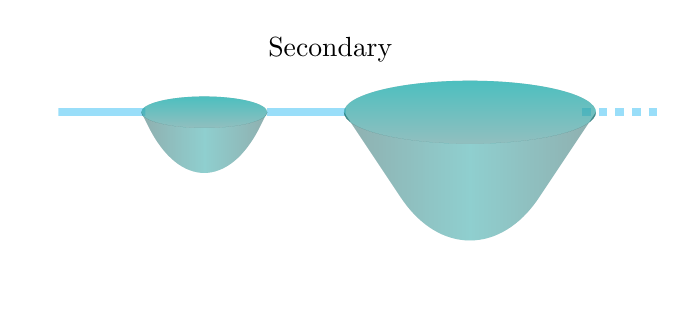
\begin{tikzpicture}[scale = 0.8]
  \draw [-,line width=3pt, cyan!40] (-1,0) to [out=0,in=180] (-2.25,0);
  \draw [-,line width=3pt, cyan!40] (1,0) to [out=0,in=180] (2.25,0);
  \draw [-,line width=3pt, dashed, cyan!40] (6,0) to [out=0,in=180] (7.25,0);
  \node at (2, 1) {Secondary};
\fill[
  top color=cyan!100,
  bottom color=cyan!40,
  shading=axis,
  opacity=0.45
  ] 
  (0,0) circle (1cm and 0.25cm);
\fill[
  left color=cyan!50!black,
  right color=cyan!50!black,
  middle color=cyan!100,
  shading=axis,
  opacity=0.25
  ] 
  (1,0) {[rounded corners=45pt] -- (0,-2)} -- (-1,0) arc (180:360:1cm and 0.25cm);
  
\fill[
  top color=cyan!100,
  bottom color=cyan!40,
  shading=axis,
  opacity=0.45,
  xshift=120
  ] 
  (0,0) circle (2cm and 0.5cm);
\fill[
  left color=cyan!50!black,
  right color=cyan!50!black,
  middle color=cyan!100,
  shading=axis,
  opacity=0.25,
  xshift=120
  ] 
  (2,0) {[rounded corners=45pt] -- (0,-3)} -- (-2,0) arc (180:360:2cm and 0.5cm);
\end{tikzpicture}
}

%%%%%%%%%%%%%%%%%%%%%%%%%%%%%%%%%%%%%%%%%%%%%%%%%%%%%%%%%%%%%%%%%%%%%%%%%%%%%%%
\section{primaryprofileblue}
\def\primaryprofileblue{
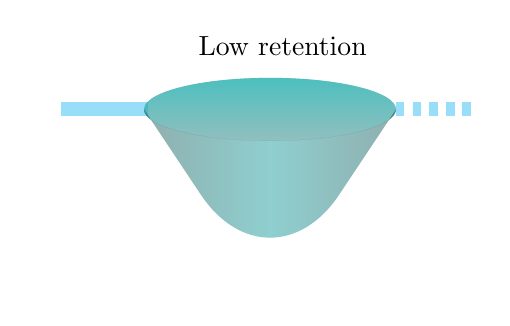
\begin{tikzpicture}[scale = 0.8]
  \draw [-,line width=5pt, cyan!40] (-2,0) to [out=0,in=180] (-3.25,0);
  \draw [-,line width=5pt, dashed, cyan!40] (2,0) to [out=0,in=180] (3.25,0);
  \node at (0.2, 1) {Low retention};
\fill[
  top color=cyan!100,
  bottom color=cyan!40,
  shading=axis,
  opacity=0.45
  ] 
  (0,0) circle (2cm and 0.5cm);
\fill[
  left color=cyan!50!black,
  right color=cyan!50!black,
  middle color=cyan!100,
  shading=axis,
  opacity=0.25
  ] 
  (2,0) {[rounded corners=45pt] -- (0,-3)} -- (-2,0) arc (180:360:2cm and 0.5cm);
\end{tikzpicture}
}

%%%%%%%%%%%%%%%%%%%%%%%%%%%%%%%%%%%%%%%%%%%%%%%%%%%%%%%%%%%%%%%%%%%%%%%%%%%%%%%
\section{primaryprofilegreen}
\def\primaryprofilegreen{
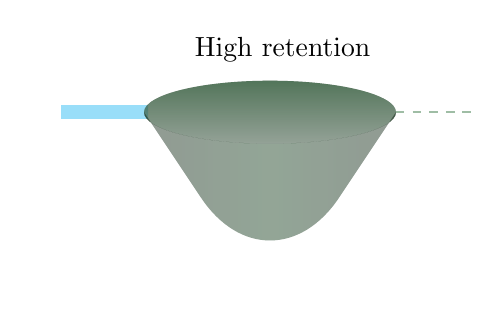
\begin{tikzpicture}[scale = 0.8]
  \draw [-,line width=5pt, cyan!40] (-2,0) to [out=0,in=180] (-3.25,0);
  \draw [-,thick, dashed, darkgreen!40] (2,0) to [out=0,in=180] (3.25,0);
  \node at (0.2, 1) {High retention};
\fill[
  top color=darkgreen!100,
  bottom color=darkgreen!40,
  shading=axis,
  opacity=0.45
  ] 
  (0,0) circle (2cm and 0.5cm);
\fill[
  left color=darkgreen!50!black,
  right color=darkgreen!50!black,
  middle color=darkgreen!100,
  shading=axis,
  opacity=0.25
  ] 
  (2,0) {[rounded corners=45pt] -- (0,-3)} -- (-2,0) arc (180:360:2cm and 0.5cm);
\end{tikzpicture}
}

%%%%%%%%%%%%%%%%%%%%%%%%%%%%%%%%%%%%%%%%%%%%%%%%%%%%%%%%%%%%%%%%%%%%%%%%%%%%%%%
\section{isolatedflux}
\def\isolatedflux[#1]#2{
\begin{tikzpicture}[scale = #1]
  \node at (1.5, 1) {#2};

\pgfsetarrowsend{latex}
\pgfsetlinewidth{1ex}

\node at (3, 5) {Evaporation};
\pgfpathmoveto{\pgfpoint{0cm}{1cm}}
\pgfpathlineto{\pgfpoint{0cm}{4cm}}
\pgfusepath{stroke}

\node at (-3, 5) {Precipitation};
\pgfpathmoveto{\pgfpoint{-1cm}{4cm}}
\pgfpathlineto{\pgfpoint{-1cm}{1cm}}
\pgfusepath{stroke}

\fill[
  top color=cyan!100,
  bottom color=cyan!40,
  shading=axis,
  opacity=0.45
  ] 
  (0,0) circle (2cm and 0.5cm);
\fill[
  left color=cyan!50!black,
  right color=cyan!50!black,
  middle color=cyan!100,
  shading=axis,
  opacity=0.25
  ] 
  (2,0) {[rounded corners=45pt] -- (0,-3)} -- (-2,0) arc (180:360:2cm and 0.5cm);
\end{tikzpicture}
}

%%%%%%%%%%%%%%%%%%%%%%%%%%%%%%%%%%%%%%%%%%%%%%%%%%%%%%%%%%%%%%%%%%%%%%%%%%%%%%%
\section{isolatedwireframe}
\def\isolatedwireframe[#1]{
\begin{tikzpicture}[scale = #1]

  % \draw[step=1cm,gray,very thin] (-4,-3) grid (4,4);

  \draw (0,0) circle (2cm and 0.5cm);
  \draw (2,0) {[rounded corners=45pt] -- (0,-3)} -- (-2,0) arc (180:360:2cm and 0.5cm);
  
  \pgfsetarrowsend{latex}
  \pgfsetlinewidth{1ex}

  \node[rotate=-90] at (0.6, 2){Evaporation};
  \node[rotate=-90] at (-0.6, 2){Precipitation};
  \node at (1.5, -2.1){Groundwater};
  \node at (-1.5, -2.1){Groundwater};
  
  
  % GW out
  \pgfpathmoveto{\pgfpoint{1cm}{-1.5cm}}
  \pgfpathlineto{\pgfpoint{2cm}{-2cm}}
  \pgfusepath{stroke}
  
  % GW in
  \pgfpathmoveto{\pgfpoint{-2cm}{-2cm}}
  \pgfpathlineto{\pgfpoint{-1cm}{-1.5cm}}
  \pgfusepath{stroke}
  
  % SW out
  % \node at (3, -0.5){Outflow};
  % \pgfpathmoveto{\pgfpoint{2.2cm}{0cm}}
  % \pgfpathlineto{\pgfpoint{4cm}{0cm}}
  % \pgfusepath{stroke}
  
  % SW in
  % \node at (-3, -0.5){Inflow};
  % \pgfpathmoveto{\pgfpoint{-4cm}{0cm}}
  % \pgfpathlineto{\pgfpoint{-2.2cm}{0cm}}
  % \pgfusepath{stroke}
  
  % Runoff in
  \node at (-3, 0.4){Runoff};
  \pgfpathmoveto{\pgfpoint{-3cm}{0cm}}
  \pgfpathlineto{\pgfpoint{-2.2cm}{0cm}}
  \pgfusepath{stroke}
  
  \pgfpathmoveto{\pgfpoint{0.26cm}{1cm}}
  \pgfpathlineto{\pgfpoint{0.26cm}{3cm}}
  \pgfusepath{stroke}
  
  \pgfpathmoveto{\pgfpoint{-0.3cm}{3cm}}
  \pgfpathlineto{\pgfpoint{-0.3cm}{1cm}}
  \pgfusepath{stroke}
  
\end{tikzpicture}
}

%%%%%%%%%%%%%%%%%%%%%%%%%%%%%%%%%%%%%%%%%%%%%%%%%%%%%%%%%%%%%%%%%%%%%%%%%%%%%%%
\section{secondarywireframe}
\def\secondarywireframe[#1]{
\begin{tikzpicture}[scale = #1]

  % \draw[step=1cm,gray,very thin] (-4,-3) grid (7,4);

  \draw [-,line width=3pt] (0,0) to [out=0,in=180] (1.25,0);
  \draw (-1,0) circle (1cm and 0.25cm);
  \draw (0,0) {[rounded corners=45pt] -- (-1,-2)} -- (-2,0) arc (180:360:1cm and 0.25cm);
  \draw[xshift=120] (-1,0) circle (2cm and 0.5cm);
  \draw[xshift=120] (1,0) {[rounded corners=45pt] -- (-1,-3)} -- (-3,0) arc (180:360:2cm and 0.5cm);
  
  \pgfsetarrowsend{latex}
  \pgfsetlinewidth{1ex}

  % GW out
  \node at (4.9, -2.1){Groundwater};
  \pgfpathmoveto{\pgfpoint{4.2cm}{-1.5cm}}
  \pgfpathlineto{\pgfpoint{5.2cm}{-2cm}}
  \pgfusepath{stroke}
  
  % GW in
  \node at (1.5, -2.1){Groundwater};
  \pgfpathmoveto{\pgfpoint{1.2cm}{-2cm}}
  \pgfpathlineto{\pgfpoint{2.2cm}{-1.5cm}}
  \pgfusepath{stroke}
  
  % SW out
  \node at (5.6, -0.5){Outflow};
  \pgfpathmoveto{\pgfpoint{5.2cm}{0cm}}
  \pgfpathlineto{\pgfpoint{7cm}{0cm}}
  \pgfusepath{stroke}
  
  % SW in
  \node at (-2.3, -0.5){Inflow};
  \pgfpathmoveto{\pgfpoint{-3.4cm}{0cm}}
  \pgfpathlineto{\pgfpoint{-2cm}{0cm}}
  \pgfusepath{stroke}
  
  % Runoff in
  \node at (-2.3, 1){Runoff};
  \pgfpathmoveto{\pgfpoint{-2.8cm}{0.6cm}}
  \pgfpathlineto{\pgfpoint{-2cm}{0.6cm}}
  \pgfusepath{stroke}
  
  % Evaporation
  \node[rotate=-90] at (3.7, 2){Evaporation};
  \pgfpathmoveto{\pgfpoint{3.36cm}{1cm}}
  \pgfpathlineto{\pgfpoint{3.36cm}{3cm}}
  \pgfusepath{stroke}
  
  % Precip
  \node[rotate=-90] at (2.4, 2){Precipitation};
  \pgfpathmoveto{\pgfpoint{2.8cm}{3cm}}
  \pgfpathlineto{\pgfpoint{2.8cm}{1cm}}
  \pgfusepath{stroke}
  
\end{tikzpicture}
}

%%%%%%%%%%%%%%%%%%%%%%%%%%%%%%%%%%%%%%%%%%%%%%%%%%%%%%%%%%%%%%%%%%%%%%%%%%%%%%%

\section{watershedconnectivity}
% See Soranno et al., 2015, Plos One
\def\watershedconnectivity[#1]{
\begin{columns}

  \begin{column}{0.7\textwidth}
    \begin{tikzpicture}[scale = #1]
      % \draw[step=1cm,gray,very thin] (-4,-2) grid (4,9);

      % streamlines
      % lake 3
        % center
      \draw [-,ultra thick, cyan] (-0.6, 3) to [out=270,in=180] (0.2,2) to [out=0,in=90] (0,0);
      \draw [-,ultra thick, cyan] (0.2, 3.2) to [out=270,in=90] (-0.1,2.2) to [out=0,in=180] (0.2,2) to [out=0,in=90] (0,0);
        % right
      \draw [-,ultra thick, cyan] (2.2,3.5) to [out=90,in=0] (1.1,1.1) to [out=270,in=90] (0,0);
        % left
      \draw [-,ultra thick, cyan] (-2.1,2) to [out=270,in=90] (-1.1,1.1) to [out=270,in=90] (0,0);

      % lake 2
      \draw [-,ultra thick, darkgreen] % 
        (-0.3,6.5) to % 
        [out=270,in=90] (0.5, 4.9) to % 
        [out=270,in=90] (0,4);

      % lakes
      \draw[cyan, ultra thick, domain=0:350, smooth cycle, fill=cyan] (0,-3) plot (\x:1+rnd*0.5);
      \node at (0, 0) {Lake 3};

      \draw[darkgreen, ultra thick, domain=0:350, smooth cycle, fill=darkgreen, yshift=4cm] (0,-3) plot (\x:1+rnd*0.5);
      \node at (0, 4) {Lake 2};

      \draw[yellow, ultra thick, domain=0:350, smooth cycle, yshift=8cm, fill=yellow] (0,-3) plot (\x:1.5+rnd*0.5);
      \node at (0, 8) {Lake 1};

      % iws
      \draw[darkgreen,ultra thick,dashed] % 
      (-1.1, 3.4) to % 
      (-1.5, 4.2) to %
      (-1.9, 5.3) to %
      (-1.5, 6.85) to %
      (-0.2, 6.1) to (0.2, 6.1) to%      
      (1.5, 6.85) to % 
      (1.9, 5.3) to %
      (1.5, 4.2) to % 
      (1.1, 3.4);      

      \draw[cyan,ultra thick,dashed] % 
      (-1.1,-0.4) to % 
      (-1.5, 0.2) to %
      (-2.5, 3) to %
      (-1.5, 6.85) to %
      (-0.2, 6.1) to (0.2, 6.1) to % 
      (1.5, 6.85) to % 
      (2.5, 3) to %
      (1.5, 0.2) to (1.1, -0.4);

      \draw [cyan, decorate,decoration={brace,amplitude=10pt,mirror,raise=4pt},yshift=0pt]
      (3,-1.5) -- (3,2.5) node [cyan,midway,xshift=0.9cm] {\footnotesize
      $IWS$};
      \draw [cyan, decorate,decoration={brace,amplitude=10pt,mirror,raise=4pt},yshift=0pt]
      (4.5,-1.5) -- (4.5,6.1) node [cyan,midway,xshift=0.9cm] {\footnotesize
      $SWS$};
      \draw [darkgreen, decorate,decoration={brace,amplitude=10pt,raise=4pt},yshift=0pt]
      (-2.5,2.5) -- (-2.5,6.1) node [darkgreen,midway,xshift=-0.8cm, align=left] {\footnotesize
      $IWS$ \\ \footnotesize $SWS$};
    \end{tikzpicture}
  \end{column}  
\end{columns}

}

%%%%%%%%%%%%%%%%%%%%%%%%%%%%%%%%%%%%%%%%%%%%%%%%%%%%%%%%%%%%%%%%%%%%%%%%%%%%%%%